\setlength{\baselineskip}{20pt}
\chapter{引言}
\label{cha:intro}

% [鼠标左键单击选择该段落,输入替换之。内容为小四号宋体。] 引言(或绪论)简要说明研究工作的目的、范围、相关领域的前人工作和知识空白、理论基础和分析、研究设想、研究方法和实验设计、预期结果和意义等。应言简意赅,不要与摘要雷同,不要成为摘要的注释。一般教科书中有的知识,在引言中不必赘述。

\section{研究背景和意义}

车联网(Internet of Vehicles,IoV)是一种基于物联网(Internet of Things,IoT)技术的智能交通系统,它通过车辆、电子、信息通信、道路交通运输等行业的深度融合,构建了一个由各种设备和异构网络组成的全球网络\cite{Architecture_Protocols_and_Security_in_IoV}。车联网是实现智能出行、智慧城市、智能物流等多种应用场景的关键技术,具有广泛的社会效益和经济价值。车联网是智能交通系统的基础和核心技术,通过车与车、车与路边单元两种通信模式,实现了移动车辆的实时感知、交通信息的协同和无线通信,提高了道路交通的安全性和效率。智能车联网不仅能够为车与车之间的间距提供保障,降低车辆发生碰撞事故的概率,还可以帮助车主实时导航与信息接收发送,通过与其他车辆和网络系统的通信实现道路环境预警。近年来,智能车联网迎来了高速发展的时代,各大汽车公式和互联网厂商都在竞相研发自动驾驶技术\cite{ref1},将车辆作为物联网的智能节点\cite{ref2}并利用无线传感器网络(WSN)实现车辆和路边设备的互联。2021年,《国家综合立体交通规划纲要》发布,将智能网联汽车、智慧交通基础设施建设作为重点任务,展现了对智能车联网的重视和支持。

然而,智能车联网也面临着严峻的网络安全挑战,因为智能网联车辆的架构日益复杂,涉及车辆、人类和其他智能设备或物品等多种网络资源\cite{Attacks_and_countermeasures_in_the_internet_of_vehicles,Attack_IOV2},车辆也集成了多种自动驾驶功能、通信接口和传感器。车端的车载网络由控制器局域网(CAN),本地互连网络(LIN),家用数字总线,FlexRay,以太网,面向媒体的系统传输,接口描述块和低压差分信号等多种异构网络组成\cite{Cybersecurity_for_autonomous_vehicles_Review_of_attacks_and_defense},这就导致了冒充攻击、GPS欺骗攻击、重放攻击、窃听攻击等安全问题在智能网联汽车上的出现\cite{ref3,ref4,Architecture_Protocols_and_Security_in_IoV},如图\ref{fig:Vehicle_networking_architecture}所示。例如,攻击者可能会通过车辆的蓝牙漏洞实现对车载网络的访问,进而控制制动等功能。因此,汽车网络安全研究需要对汽车的设计、架构、功能、攻击面有一个宏观性的理解。由于传统的网络安全研究人员往往都没有参与过汽车的设计、研发、生产,对于汽车的了解仅限于其表面的功能表现,而汽车又是当今最复杂的工业制造产品之一,因此车联网安全是当今的研究热点。为了保障智能网联汽车的安全性和可靠性,本文从网络安全的角度,分析智能车联网的安全需求、安全威胁和安全防护,提出了一套针对车联网的安全解决方案,旨在为智能车联网的发展和应用提供理论和技术支持。

\begin{figure}[htb]
    \centering
    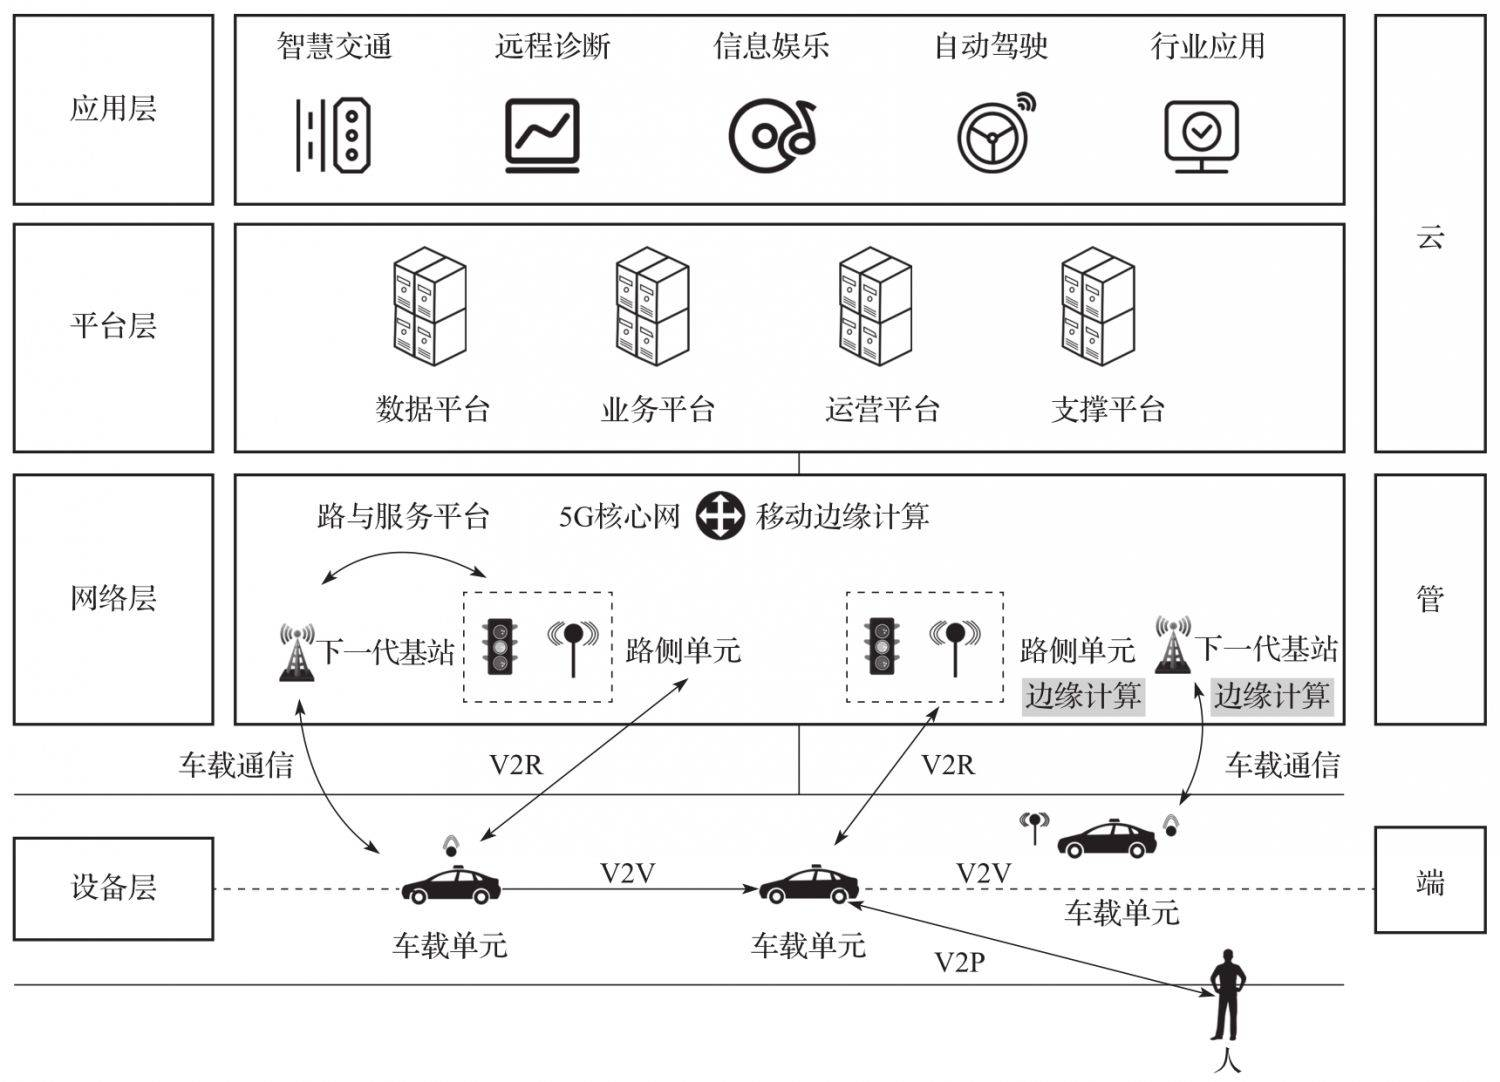
\includegraphics[width=0.95 \textwidth]{figures/chapter1/chapter1.4.jpg}
    \caption{从网络安全角度分析车联网架构}
    \label{fig:Vehicle_networking_architecture}
\end{figure}

当今时代,汽车行业没有出于安全原因限制互联网连接,反而出于商业原因继续增加互联网连接,在没有充分安全保障的情况下将新设备和新功能匆忙推向市场。同时,汽车系统里使用了大量无法保证安全性的开源软件,这使安全问题进一步加剧。英特尔的一项研究表明,如果只考虑自动驾驶专用传感器,仅一辆自动驾驶汽车每天就会产生大约4000GB的数据,每年产生的数据量更是惊人。汽车中的数据生成和收集并不是一个新现象。例如,为了有助于分析碰撞或技术故障,制造商需要记录事件数据和车载诊断数据。欧洲要求于2022年3月起新车强制安装EDR,存量车于2024年3月起安装。这些设备应该通过匿名存储事故数据来确定事故发生的原因,为事后调查提供数据支撑,类似于飞机上的黑匣子。过去几年的技术进步导致汽车收集的数据量和种类激增。汽车不仅是将驾驶员和乘客从A点带到B点的交通工具,而且也是一种智能设备,所以将装有传感器的汽车放在道路上存在隐私问题。汽车不仅会收集驾驶员和乘客的信息,还会收集周围的车辆、行人和城市的信息以及国家测绘数据。车联网中的数据隐私泄露与攻击行为不仅会侵犯车主和乘客的个人隐私,还会危害国家安全和社会稳定。例如,如果攻击者能够获取车辆的位置、速度、行驶路线等信息,就可能对车辆进行跟踪、拦截、劫持等恶意行为;如果攻击者能够获取车辆的控制权,就可能对车辆进行篡改、破坏、制造事故等恶意行为;如果攻击者能够获取车辆的通信内容,就可能对车辆进行监听、干扰、欺骗等恶意行为。这些恶意行为不仅会威胁车辆的正常运行,还会危害车主和乘客的生命财产安全,甚至会影响整个交通系统的稳定性。因此,本文将针对车联网的数据隐私泄露与攻击行为提出相应的保护措施。

车联网中广泛应用了深度学习(DL)模型,以提升车辆的智能化和个性化。例如,通过摄像头或者雷达等传感器,对车辆周围的道路环境进行识别,帮助车辆实现自动驾驶、车道保持、碰撞预警等功能的模型,如YOLO、Mask R-CNN、LaneNet等;通过语音或者手势等方式,与车主或者乘客进行交互,提供娱乐、导航、信息等服务的模型,如Alexa、Siri、斑马智行等;通过无线网络,与其他车辆或者路边设备进行通信,实现数据的交换和协同,提高车辆的安全性和效率,实现智能交通和车队管理等功能的模型,如V2X、C-V2X、DSRC等。然而,DL模型的性能依赖于训练数据集的规模和质量,而训练数据集中可能包含大量的敏感信息,攻击者可以通过逆向手段还原出训练数据集,从而泄露用户隐私。例如,公安机关发布的犯罪嫌疑人识别模型,其训练数据集包含了全国人口的图像信息,如果攻击者能够还原出训练数据集中的图像,就会暴露个人敏感信息。因此,如何在保护个人敏感信息的同时,提高数据的可用性,是DL应用面临的一个主要问题,也是DL未来发展和应用的一个重要因素。本文针对车联网中的隐私安全问题,提出了一种基于联邦学习的车联网异常检测方法,将车联网中的隐私安全分为数据安全与模型安全两部分。数据安全主要涉及车联网中的数据采集、存储、传输和处理过程中的隐私保护,包括数据的加密、匿名化、脱敏等技术。模型安全主要涉及车联网中的DL模型的训练、部署和使用过程中的隐私保护,包括模型的加密、混淆、防篡改等技术。数据安全和模型安全是车联网中的隐私安全的两个重要方面,缺一不可。

% \begin{figure}[htb]
%     \centering
%     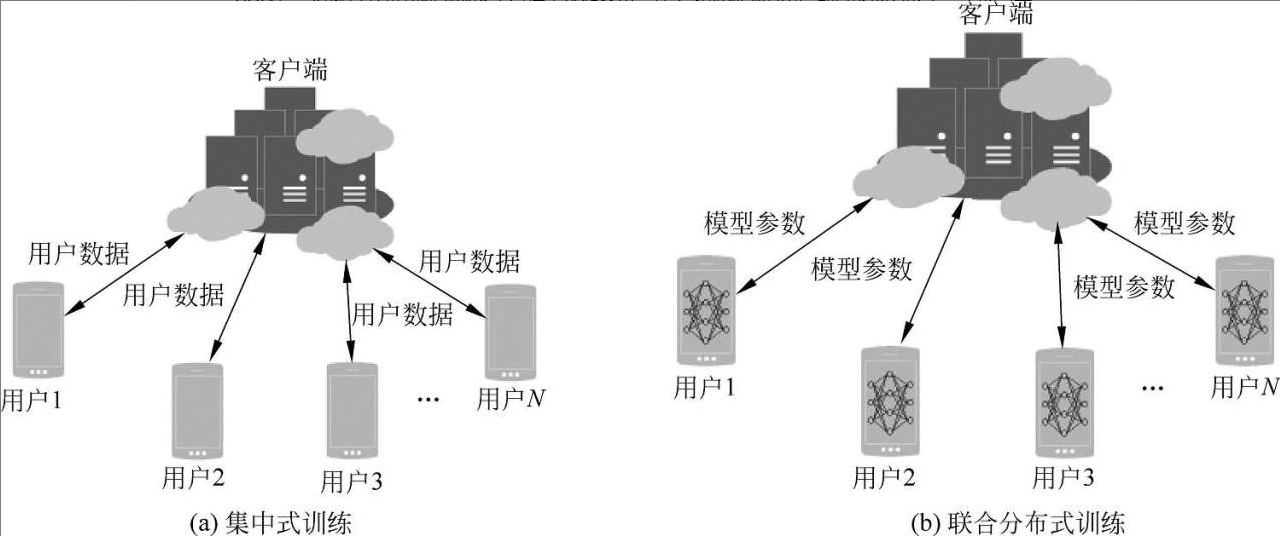
\includegraphics[width=0.85 \textwidth]{figures/chapter1/chapter1.1.png}
%     \caption{协作学习的两种威胁模型}
%     \label{fig:Two_threat_models_of_collaborative_learning}
% \end{figure}

% 将协作性模型与DL结合起来,可以通过多个数据源之间的协作来训练更加精确的协作性DL模型,在保证不同企业之间数据独立性的基础上,不同的企业之间可以实现模型的共享,任何一个模型学习到的知识都可以及时地共享给其他协作的企业,使所有企业都能从中受益。然而,协作性模型仍然会面临模型反演攻击、污染攻击等隐私窃取攻击的威胁。同时,一些领域对数据机密性的要求较高,比如在网络空间安全领域,如果遭受攻击,像入侵检测中用到的流量数据,会暴露目标网络的一些重要的配置信息;网站的请求数,会暴露网站架构以及用户的一些敏感隐私内容,同时,DL模型会无意中记录一些训练数据,而一些训练数据涉及人们的隐私,如习惯、爱好、地理位置等。在DL模型应用的健康系统中,隐私威胁不仅泄露患者隐私,攻击者可能发起攻击修改患者的用药剂量导致患者生命危险。因此安全厂商对于数据的机密性保护给予了高度重视。图\ref{fig:Deep_learning_model_training_methods}给出了常见的隐私窃取方式,这些隐私威胁分别针对机器学习过程中的训练阶段和预测阶段。
% \begin{figure}[htb]
%     \centering
%     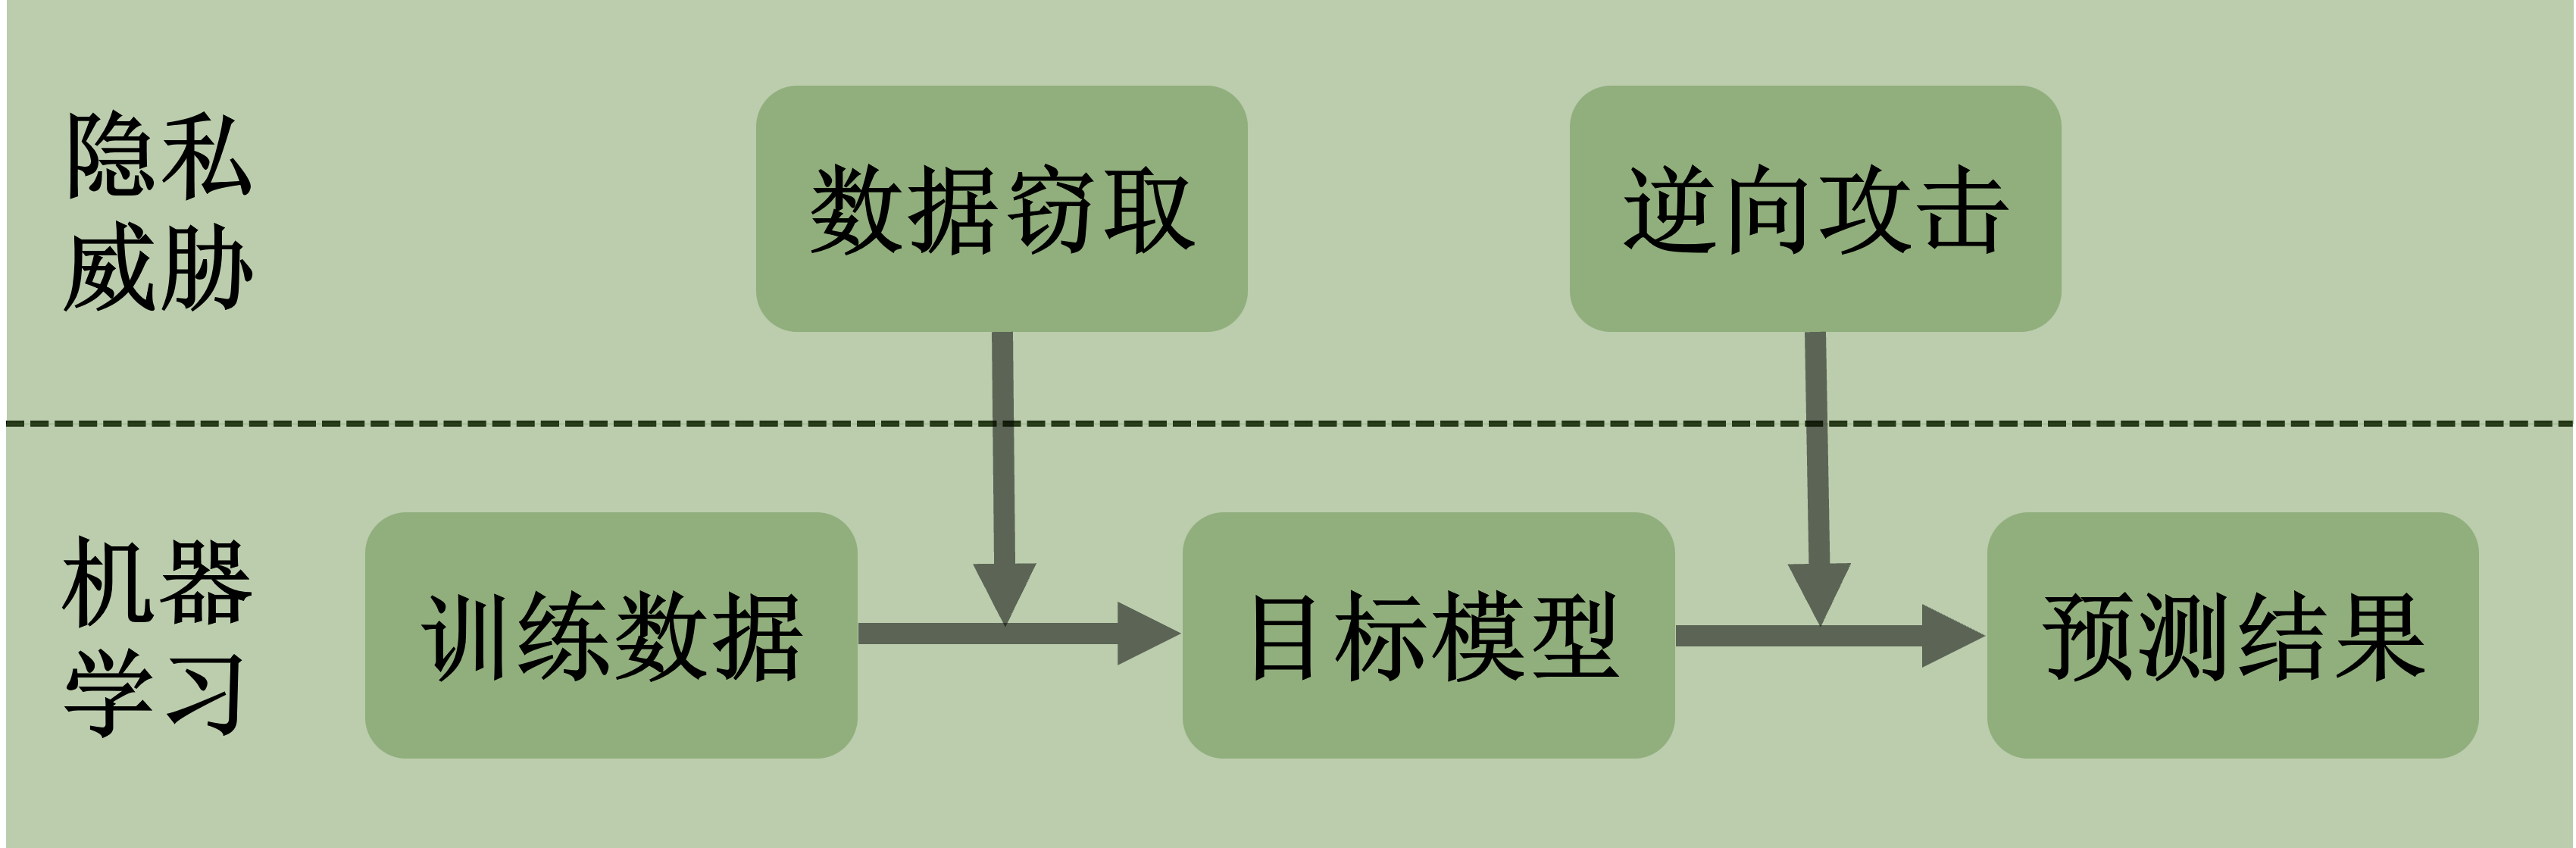
\includegraphics[width=0.55 \textwidth]{figures/chapter1/chapter1.png}
%     \caption{深度学习模型训练方式}
%     \label{fig:Deep_learning_model_training_methods}
% \end{figure}

% 传统的机器学习模式要求在模型训练之前将数据汇总到中心。但是,当数据偏离原有的数据域后,数据可能会变得无法控制,从而导致数据隐私泄露和数据安全风险。联邦学习是谷歌提出的一种分布式机器学习技术。与传统的机器学习不同,它不需要将数据集中在单个中心,从而支持分布式协作训练模型和保护数据隐私。由于其保护隐私和去中心化的内在特点,FL得到了各行各业的广泛青睐。对于大规模深度神经网络训练,联邦学习最近已成为分布式随机优的常见实现\cite{Gradient_Leakage_Attacks_in_Federated_Learning}。然而,大量研究表明联邦学习仍然存在大量安全问题,例如投毒攻击、对抗性样本攻击、隐私泄露等。在隐私泄露中,除了窃取模型之外,还可以从联邦训练中收集统计信息\cite{Safeguard_the_Original_Data_in_Federated_Learning_via_Data_Decomposition}。机器学习训练方式分为集中式和联合分布式,如图4-6所示。大型公司多用集中训练方式,因为拥有足够多的用户便于搜集大量的训练数据。在搜集用户数据过程中,会暴露一些用户的隐私,Google和Apple公司采用差分隐私的方式保护用户数据,在用户数据中,加入噪声使单一的数据没有现实意义,而统计信息具有应用价值。为了扩大训练数据集得到精确的目标模型,一些数据提供方需要进行协作“分享”数据,共同训练目标模型。“分享”不是直接对其他参与方公开数据,各个参与方独自在各自数据集上训练自己的模型,与其他参与方共享训练结果,从而间接分享各自的训练数据。

\section{研究内容及贡献}

本文旨在利用隐私保护策略,提高车联网中数据和模型的安全性,设计并实现了一种基于CAN总线的异常检测系统和一种基于稀疏学习和梯度扰动的梯度泄露防护方案。基于联邦学习的车联网异常检测系统的研究内容框架如图\ref{fig:Anomaly_detection_system_of_IoVFL}所示。本文的研究内容分为两个部分:第一部分是基于联邦学习的车联网CAN异常检测,通过构建多方参与的联邦学习模型,实现对车辆行驶状态的实时监测和异常识别;第二部分是基于稀疏学习和梯度扰动的梯度泄露防护方案,通过引入稀疏约束和随机扰动,降低联邦学习中梯度信息的可逆性和可推断性,保护参与者的隐私数据。下面将对将对数据安全和隐私保护的研究内容进行详细的介绍。

\begin{figure}[htb]
    \centering
    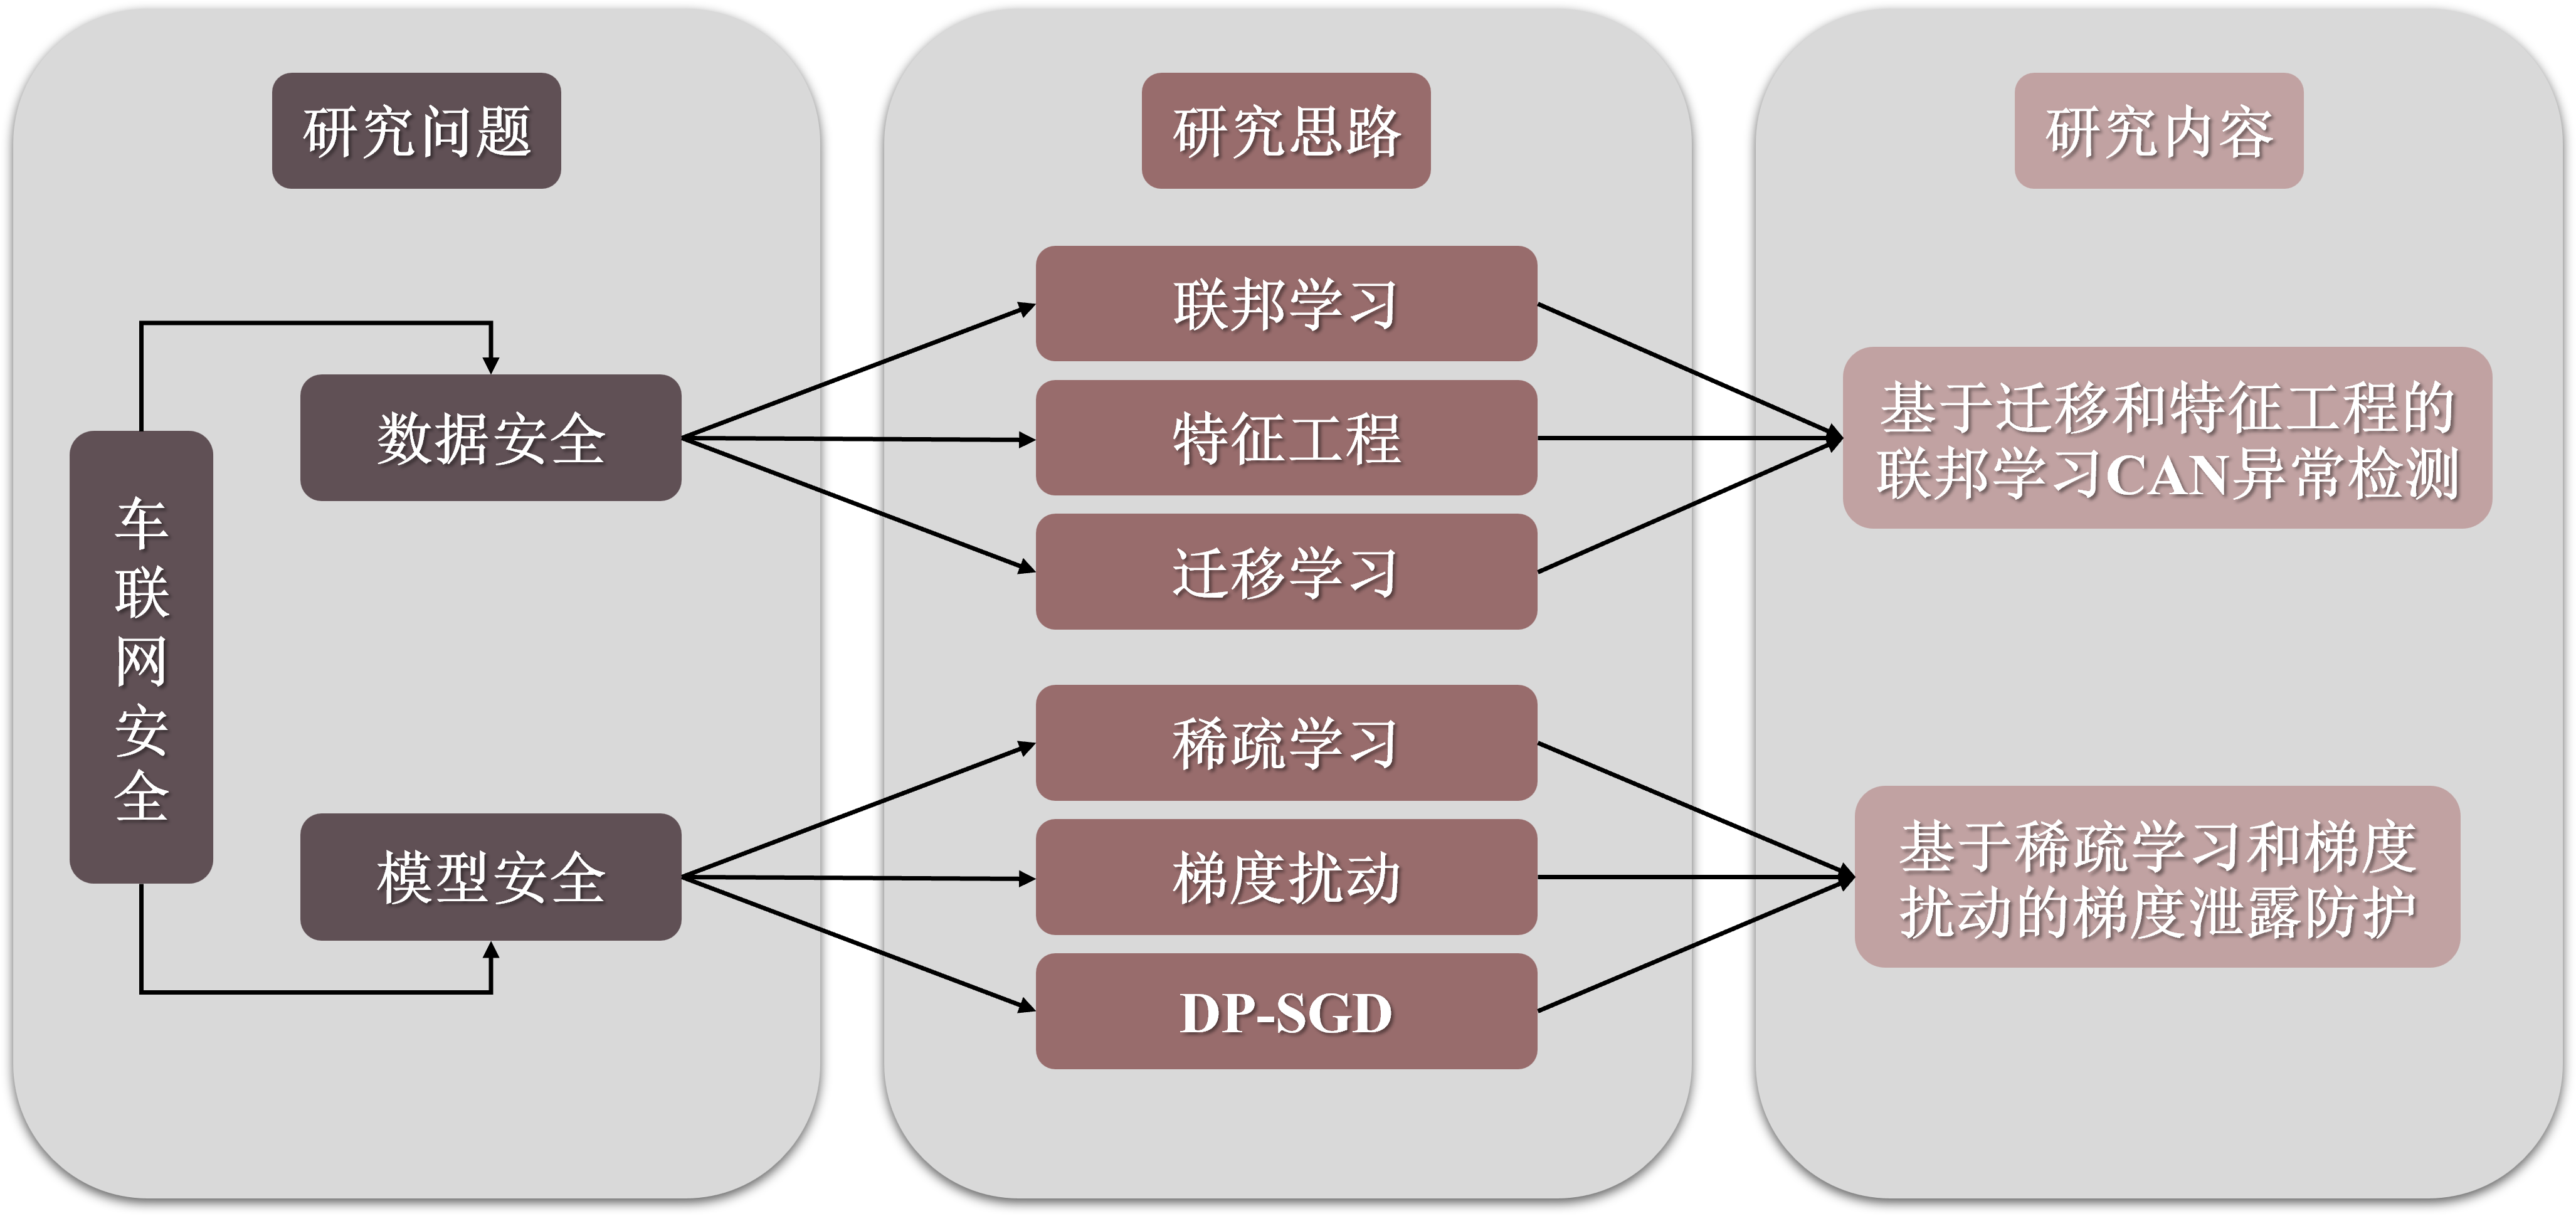
\includegraphics[width=1 \textwidth]{figures/chapter1/chapter1.2.png}
    \caption{基于联邦学习的车联网异常检测系统}
    \label{fig:Anomaly_detection_system_of_IoVFL}
\end{figure}

车联网利用IEEE802.11p协议构建了一个由车辆和路边基础设施组成的分布式网络,能够管理车辆及其相关网络产生的数据,并为交通管制、公共保护等各种服务提供数据支持\cite{ref5,Data_communication_in_VANETs}。本文将车联网中的攻击分为两类:一类是恶意的外部攻击,另一类是系统故障。恶意的外部攻击是指那些利用车辆或路边设备的漏洞,对车联网的功能和安全造成破坏的攻击。本文假设车辆的制造商以及RSU等相关设备的生产者是友善的,他们不会故意在制造过程中留有后门,因此,单个车辆和单个RSU都是友好而积极的参与者,车辆内部系统不存在恶意的破坏者。系统故障是指那些由于开发者的粗心或者其他原因,导致车辆或路边设备的软件或硬件出现异常的情况。一旦系统故障发生,系统中的参与者无法为其他参与者提供服务,在其他参与者眼中,其状态为离线。本文的第一个研究点是来自车辆内部的攻击,这类攻击会破坏系统功能,不仅危及驾驶者的安全,而且可能对公司财务和运营、乘客的隐私等方面造成影响\cite{ref6}。攻击者可以干扰智能车辆内部的通信,使其无法获取道路信息,例如利用BSM(Basic Safety Messages)发动的攻击\cite{Message_Sieving_to_Mitigate_Smart_Gridlock_Attacks_in_V2V},或者基于认知无线电(CR)的频谱感知数据伪造(SSDF)攻击和主用户仿真(PUE)攻击\cite{Defense_against_SSDF_Attack_and_PUE_Attack_in_CR-Internet_of_Vehicles_(IoVs)_for_Millimeter_Wave_Massive_MIMO_Beamforming_Systems}。由于车辆由多个组件构成,例如车辆机器、内部网关和控制器,它们的编译环境、操作系统和传输协议各不相同,现有的网络入侵检测系统无法完全预防和隔离针对车辆的威胁\cite{CANintelliIDS_Detecting_In-Vehicle_Intrusion_Attacks_on_a_Controller_Area_Network_Using_CNN_and_Attention-Based_GRU},例如破坏多传感器融合(MSF)算法的FusionRipper攻击\cite{Drift_with_Devil_Security_of_Multi-Sensor_Fusion_based_Localization_in_High-Level_Autonomous_Driving_under_GPS_Spoofing}。车内网络也容易受到攻击,黑客可以通过攻击CAN总线控制车辆主控制器,导致事故,例如针对CAN总线的攻击\cite{Cloaking_the_Clock_Emulating_Clock_Skew_in_Controller_Area_Networks,A_Survey_on_Controller_Area_Network_Reverse_Engineering,Implementation_of_a_bluetooth_attack_on_controller_area_network_CAN}。

本文对车内攻击的研究重点就是CAN总线。控制器局域网(CAN)总线是一个低容错的协议,主要用于ECU和车载汽车网络的实时通信\cite{Intrusion_Detection_System_CAN-Bus_In_Vehicle_Networks_Based_on_the_Statistical_Characteristics_of_Attacks},它具有低成本、抗噪和容错性高等特点,被广泛应用于车载网中。由于CAN发送的是实时性很高的报文,因此并不适合引入重安全机制。而入侵检测系统(IDSs)是一种预防性保护机制,可以在软件完整性验证\cite{ref9}之后作为第二道防线,实现持续性的事件监控\cite{ref10}。在车联网中使用IDSs可以非侵入性地运行,最小化对车联网的影响,同时IDSs可以与人工审计结合提醒安全人员注意潜在的威胁,以便他们能够更有效地保护客户的车辆免受威胁\cite{ref11}。然而,将传统入侵检测系统引入车联网领域将面临多种问题,首先是数据量爆炸问题,车联网中的节点可能在计算和内存方面受到限制。然而,深度学习模型的训练过程中,无论是数据采样还是分析,都将消耗大量的节点资源。因此,需要考虑模型对智能车带来的性能消耗问题。其次,车联网的动态性问题,车联网与物联网的一大区别就在于车辆的动态性,这意味着整个车联网的拓扑结构是频繁变化的,车辆节点接入网络具有随机性\cite{Attack_IOV2},这将导致不同地区的RSU所拥有的网络质量、收到的数据量等客观条件之间有较大的差异,然而,深度学习模型的检测性能与这些数值高度相关。这两个都可以归类为数据的非独立同分布问题。

车联网是一种利用车辆和路边基础设施之间的通信来提供智能交通服务的网络。车联网中的车辆可以收集和处理各种数据,例如位置、速度、方向、路况、天气、驾驶行为等,从而提高道路安全和效率,降低能耗和污染,增强驾驶体验和舒适度。为了实现这些目标,车联网中广泛使用了深度学习(DL)算法,例如卷积神经网络(CNN)、循环神经网络(RNN)、长短期记忆网络(LSTM)等,来处理图像、语音、文本、视频等多模态数据。然而,这些DL算法也带来了隐私和安全的挑战,因为它们可能会泄露训练数据的敏感信息。恶意的攻击者可以利用这些DL算法中泄露出来的梯度,通过一些逆向工程的技术,反推出原始数据,从而侵犯用户的隐私。例如,攻击者可以通过梯度重构攻击(GRA)\cite{Model_Inversion_Attacks_that_Exploit_Confidence_Information_and_Basic_Countermeasures},从梯度中恢复出图像或文本数据;或者通过成员推理攻击(MIA)\cite{Membership_Inference_Attacks_Against_Machine_Learning_Models},从梯度中判断某个数据是否属于训练集;或者通过属性推理攻击(AIA)\cite{Property_Inference_Attacks_on_Fully_Connected_Neural_Networks_using_Permutation_Invariant_Representations},从梯度中推断出某个数据的某个属性,例如性别、年龄、疾病等。这些攻击不仅威胁到用户的个人隐私,而且可能导致法律、道德、社会等方面的问题。因此,如何防御梯度泄露攻击,保护车联网中用户的隐私,是一个亟待解决的研究问题。

本文对DL模型攻击研究的重点是梯度泄露攻击(DLG),一种针对联邦学习系统的隐私攻击,它利用了参与者之间共享的梯度信息,来推测或重构出原始的训练数据。联邦学习是一种分布式机器学习的方法,它允许多个参与者在不共享数据的情况下,通过交换本地模型的更新来联合训练一个全局模型。这种方法被认为可以保护参与者的数据隐私,但是实际上,梯度中可能包含了训练数据的敏感信息,例如标签、属性、图像等。梯度泄露攻击的基本思想是,给定一个预训练的模型和一个共享的梯度,攻击者可以随机生成一对伪输入和标签,然后将其输入模型并计算伪梯度。接着,攻击者可以优化伪输入和标签,使得伪梯度和真实梯度之间的距离最小化。这样,伪输入和标签就会逐渐接近原始的训练数据。当优化过程完成后,攻击者就可以从伪输入和标签中获取私有的数据。这种攻击可以应用于不同的数据类型和模型结构,例如图像、文本、全连接层、卷积层等。梯度泄露攻击的危害范围很大,它可以影响中心化和去中心化的联邦学习系统。在中心化的系统中,参数服务器可以从每个参与者的梯度中窃取其本地训练数据。在去中心化的系统中,任何一个参与者都可以从与其交换梯度的其他参与者中窃取其训练数据。这些攻击不仅威胁到参与者的个人隐私,而且可能导致法律、道德、社会等方面的问题。梯度泄露攻击的防御方法有一些,例如梯度压缩、梯度噪声、差分隐私等。这些方法都有一定的效果,但也会带来一些性能损失或计算开销。

针对上述问题,本文所做的工作如下:

(1)为了解决车联网数据安全问题,本文提出了一种基于迁移和特征工程的联邦学习CAN异常检测。该系统采用联邦平均算法进行全局模型训练,只需在参与者之间交换本地模型的梯度,无需共享原始数据,从而节省了车联网的传输带宽。该系统还结合了迁移学习的思想,将CNN、VGG16、AlexNet、ResNet18等四种深度学习算法融合到联邦学习中,为用户提供了多种选择,同时减少了训练成本和数据需求。此外,针对车联网的动态性导致的数据异构问题,本文提出了一种针对CAN总线数据的特征工程方案,以提高分类模型的性能。最后,本文通过实验验证了所提出的模型的有效性。仿真结果显示,本文设计的框架能够显著提升车联网的安全性。

(2)为解决车联网中的模型安全问题,提出了一种基于稀疏学习和梯度扰动的梯度泄露防护方案。该方案的主要思想是,在RSU接收到训练数据之前,利用稀疏学习的方法,对原始数据进行系数学习和稀疏化处理,从而降低数据中的敏感信息泄露风险。在MEC进行全局模型训练时,从模型中提取表示层,根据表示层的$L_2$范数计算梯度筛,然后将梯度筛应用到表示层中,使得筛出来的部分梯度加上拉普拉斯噪声,从而扰乱表示层梯度中的信息。本文通过实验评估了所提出方案的有效性,结果表明,该方案能够有效地防止梯度泄露攻击,同时保持模型的性能。

\section{论文组织结构}

本文一共分为五章,具体内容如下: 

第一章\ 引言

本章主要介绍本文的研究背景、内容和框架。首先,从车联网目前面临的安全问题出发,分析了数据安全和模型安全在车联网应用场景中的重要性和挑战。其次,概述了本文的主要研究内容,包括车联网数据安全和模型安全的研究问题、方法和贡献。最后,说明了本文的组织结构和章节安排。

第二章\  研究现状

本章主要介绍车联网异常检测和梯度泄露的研究现状,分为两个部分:一是车联网数据安全的入侵检测系统(IDS)的发展现状,从基于普通深度学习算法的IDS、基于高级深度学习算法的IDS和关注于数据隐私保护的IDS三个角度进行分析;二是车联网模型安全的梯度泄露的发展现状,从基于优化的梯度泄露攻击和梯度泄露防御两个方面进行介绍。

第三章\  基于迁移和特征工程的联邦学习CAN异常检测

本章主要介绍了一种针对车联网安全中的数据安全问题而提出的有效方法,即基于迁移学习和特征工程的联邦学习CAN异常检测设计框架。首先,本章对相关工作和技术进行了简要的说明,其中涉及到了联邦学习、迁移学习和特征工程的技术原理。其次,本章对所提出的基于迁移和特征工程的联邦学习CAN异常检测框架进行了详细的阐述,包括了车辆与RSU之前的数据传输、RSU上的DL模型选择、MEC上的联邦学习等策略。最后,本章对说提出框架进行了实验测评和性能分析,验证了所提出框架的有效性和优越性。最后,本章对基于迁移和特征工程的联邦学习CAN异常检测的主要内容进行了总结和归纳。

第四章\  基于稀疏学习和梯度扰动的梯度泄露防护 

本章主要介绍了一种针对车联网安全中的模型安全问题而提出的有效的方法,即基于稀疏学习和梯度扰动的梯度泄露防护方法。首先,本章对相关的工作和技术进行了简要的说明,其中涉及到了特征提取与稀疏学习的相关概念和技术原理,以及差分隐私的相关概念和技术原理。其次,本章对所提出的基于稀疏学习和梯度扰动的梯度泄露防护方案进行了详细的阐述,包括了梯度泄露攻击模型的形式化定义、基于稀疏学习的数据隐私保护策略的具体实现和基于DP-SGD的梯度扰动策略的具体实现。最后,本章对所提出的方法进行了实验测评和性能分析,验证了所提出方法的有效性和优越性。最后,本章对基于稀疏学习和梯度扰动的梯度泄露防护方法的主要内容进行了总结和归纳。

第五章\  结论和未来工作 

本章总结了基于联邦学习的车联网异常检测系统的研究成果和展望。首先回顾了车联网数据安全和模型安全的问题及本文提出的解决方案,然后指出了本文的不足之处和改进方向,并提出了未来的研究计划。
